\documentclass[../main.tex]{subfiles}
\chapter{Validierung}
\label{c:validierung}

Die Beschreibung der Kinematik der Maschine erfolgt mit einer homogenen Transformationsmatrix je Freiheitsgrad.
Die der Simulation zugrunde liegende Maschine hat 6 geführte Freiheitsgrade.
Von diesen sind 4 über einen Vorschub an die Drehzahl des Werkzeugs gekoppelt.
Die positive Richtung dieser Freiheitsgrade ist außerdem nicht streng anhand der mathematisch positive Richtung des Standardkoordinatensystems definiert.
Um Vorzeichen-, Drehmittelpunkts- und Fehler in der Anwendungsreihenfolge der Abbildungsmatrizen zu verhindern ist eine visuelle Validierung der in Kap.\ \ref{c:herleitung} entwickelten linearen Algebra anhand einer erprobten Methode also sinnvoll.
Diese Methode sollte Teil der \matlab Toolchain sein, erlauben das Modell extern zu bedaten und eine grafische Ausgabe zur Verfügung stellen.
Es wurde entschieden das kinematische Modell als Simscape Multibody Modell aufzubauen.
Bei Simscape\texttrademark\xspace handelt es sich um eine Reihe von Blockbibliotheken und speziellen Simulationsfunktionen zur Modellierung physikalischer Systeme in der Simulink\textregistered-Umgebung.
Sie verwendet den Physical Network-Ansatz, der sich von dem Standard-Simulink-Modellierungsansatz unterscheidet und sich besonders für die Simulation von Systemen eignet, die aus realen physikalischen Komponenten bestehen. \cite{mwSim}
Vergleichbar zu Simulink wird hier ein Signalflussplan erstellt, der die Wechselwirkung von, zu Blöcken zusammengefassten, Funktionsgruppen mit Hilfe von Verbindungen beschriebt.
Diese Verbindungen stellen in Simulink Signale dar, üblicherweise zeitdiskrete Zahlenwerte oder logische Zustände.
In Simscape stellen diese Verbindungen allerdings die Position und Ausrichtung eines Koordinatensystems im Raum dar.
Diese verschiedenen Formen der Modellierung können in einem Blockschaltbild koexistieren und mit Hilfe von ,,Physical Signal Converters'' vereint werden.
So kann ein Simulink-Signal in eine zeitdiskrete Transformation eines Koordinatensystem gewandelt werden, oder Position und Ausrichtung eines Koordinatensystems in einem Signal erfasst werden.

\section{Mechanisches Modell der Maschine}

Anhand der schematischen Darstellung einer Wälzfräsmaschine in Abb.\ \ref{fig:maschine} wurde in Creo Parametric ein dreidimensionales Modell erstellt.
Die Komponenten der Maschine wurden im Mechanismus-Modus zu einem kinematischen Modell verknüpft.
Dieses kinematische CAD-Modell wurde anschließend mittels einer Softwareschnittstelle in ein Simscape Multibody Modell konvertiert.

Ursprung des CAD-Modells ist das Maschinenbett-Koordinatensystem.
Anfänglich wurden alle Komponenten der Maschine auf dieses Standard-Koordinatensystem konstruiert.
Nach Konvertierung der CAD-Komponenten in ein neutrales Datenformat beinhalten alle Teile dieses Koordinatensystem als Ursprung.
Dadurch sollte der Aufbau des Simscale Modells vereinfachen werden, da alle Komponenten ohne linearen oder rotatorischen Versatz auf des world-Koordinatensystem referenziert werden können.

\begin{figure}
	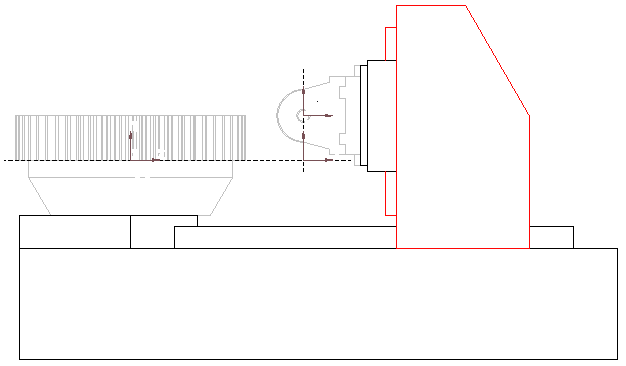
\includegraphics{skelettmodell}
	\caption{Konstruktion des Koordinatensystems für Schlitten in x-Richtung}
	\label{fig:skelettmodell}
\end{figure}

Die in Simscape zur Verfügung stehenden Blöcke verwenden als primäre Achse allerdings immer die z-Achse; Translationen können ausschließlich entlang der z-Achse erfolgen, Rotationen ausschließlich um diese herum.
Es ist also notwendig, den Komponenten zweckmäßige und individuelle Koordinatensysteme aufzuprägen.
Als Ursprung für ein solches Koordinatensystem bietet sich der Schnittpunkt von Hauptachsen der Koordinatensysteme der Mutter- und Tochter-Komponenten (vgl. Abb.\ \ref{fig:skelettmodell}) an.
Die Ausrichtung sollte mit Blick auf die Transformation der Tochter-Komponenten so gewählt werden, dass keine weitere Transformation innerhalb der Komponente notwendig ist.
In Abbildung \ref{fig:skelettmodell} ist die Konstruktion des Koordinatensystems für den Maschinenschlitten der x-Achse (mit roter Umrandung) dargestellt.
Das in der kinematischen Kette vor dieser Komponente liegende Bauteil, das Maschinenbett, übergibt ein Koordinatensystem mit z-Achse in Richtung des x-Achsen-Freiheitsgrades.
Das Koordinatensystem muss also um einen Offset verschoben und so gedreht werden, dass die z-Achse auf der Ausgangsseite in Richtung des Maschinen-Z-Freiheitsgrades zeigt.
Das Koordinatensystem des in der kinematischen Kette nachfolgend liegende Teiles, der Schlitten der z-Achse ist dann wiederum translatorisch verschoben, damit der Ursprung auf der Rotationsachse der Werkzeugspindel liegt.
Dieses muss dann im nächsten Schritt noch so gedreht werden, dass die z-Achse in Richtung der Rotationsachse der A-Achse zeigt.

Eine mechanische Komponente wird innerhalb von Simscape als ,,File Solid'' Block repräsentiert.
Dieser Block hat, wie andere mechanische Blöcke, einen Koordinatensystem-Eingang und es können ein oder mehrere Ausgänge ergänzt werden.
Maskiert innerhalb des Blockes kann eine feste Transformation von Eingang zu Ausgangskoordinatensystem definiert werden.
Als Ursprung eines sekundären Koordinatensystems kann lediglich ein Koordinatensystem, der Massenschwerpunkt des Körpers sowie der Flächenschwerpunkt einer frei wählbaren Fläche, nicht etwa ein definierbarer Punkt im Raum.
Es ist also notwendig, solche Koordinatensysteme bereits im CAD vorzusehen.

\section{Aufbau des Simscape Multibody Modells}

\begin{figure}
	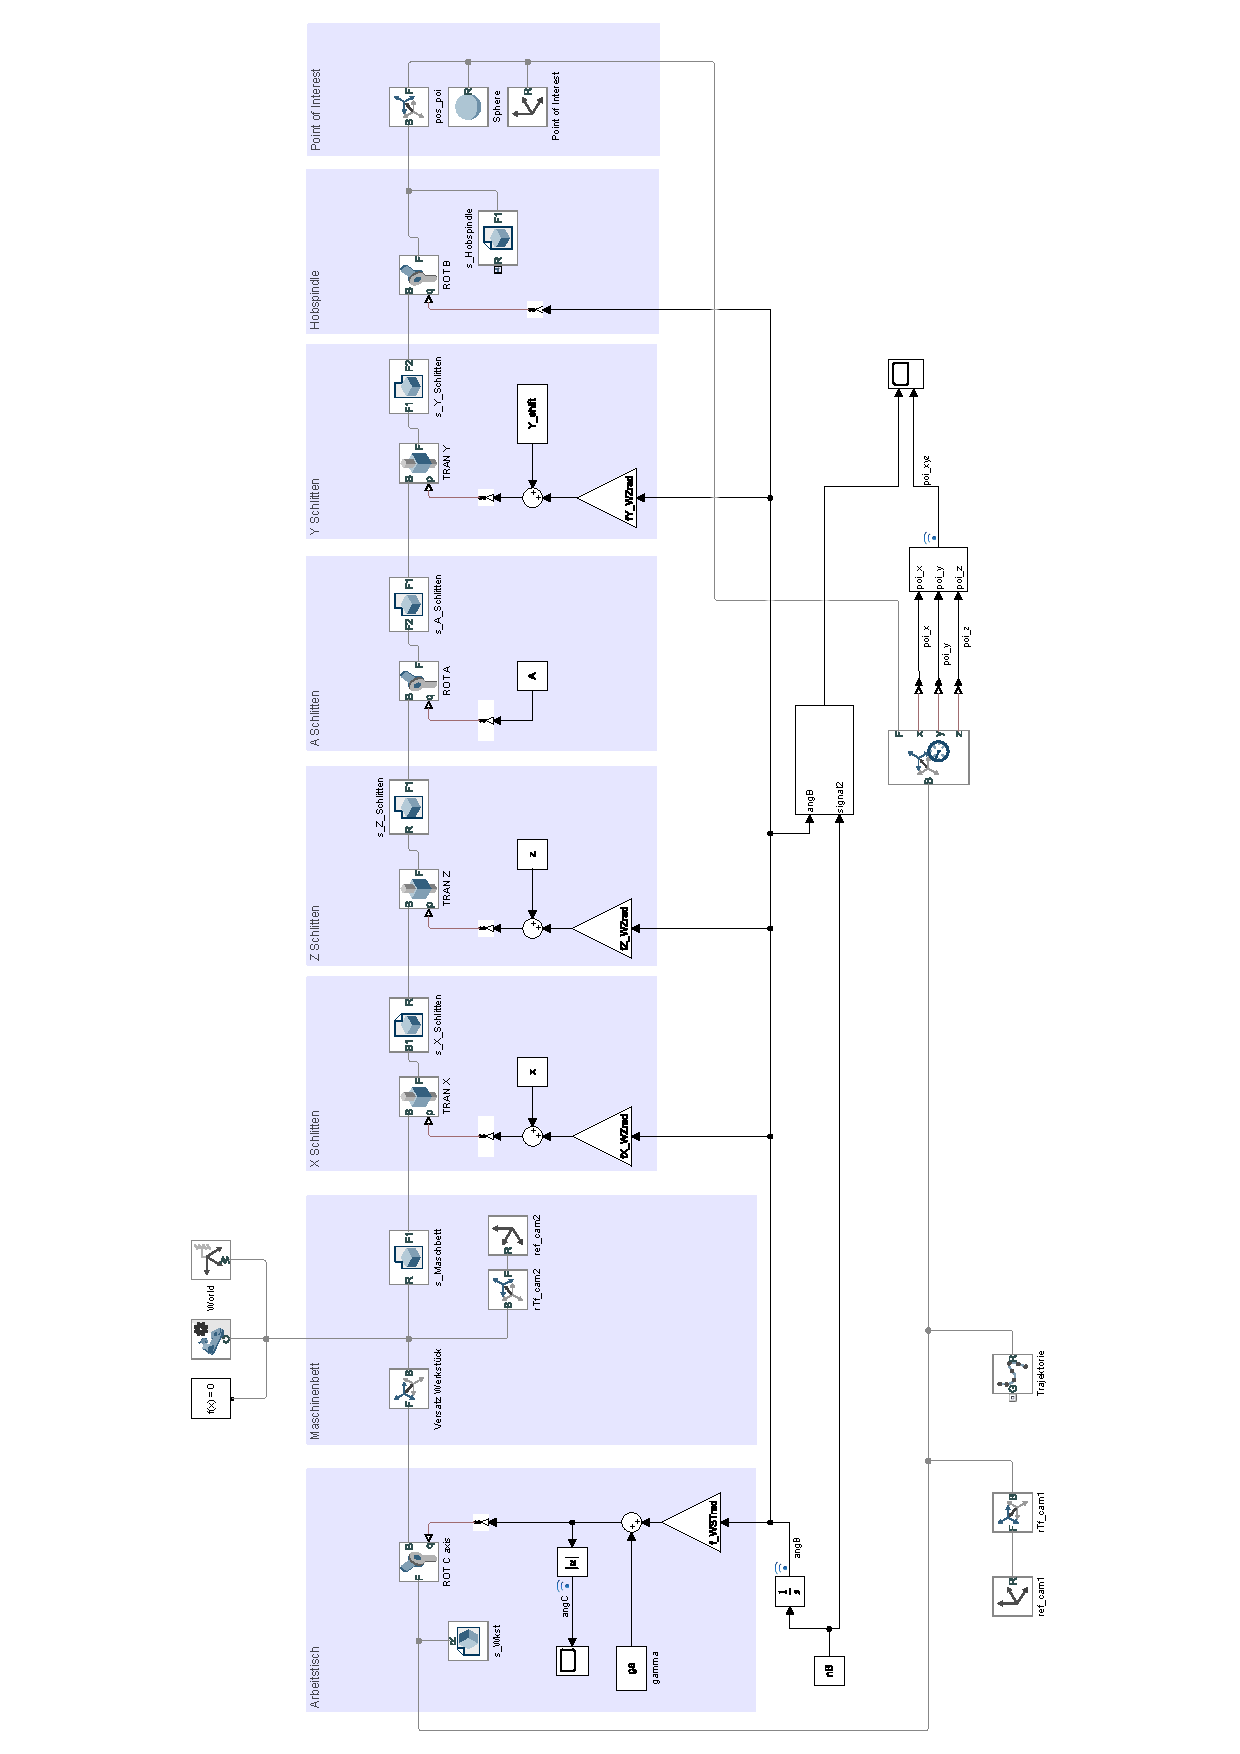
\includegraphics[scale=0.75]{simscapemdl}
	\caption{Signalflussplan des Simscape Modells}
	\label{fig:simscapemdl}
\end{figure}

Abbildung \ref{fig:simscapemdl} zeigt den Signalflussplan des zur Validierung eingesetzten Simscape Modells.
Ausgehend vom Ursprung des Modells, das ,,world''-Koordinatensystem, breiten sich die gleichen zwei Pfade aus, die weiter oben bereits beschrieben wurden.

Im Werkstück-Pfad muss zunächst der Versatz des Bearbeitungstisches berücksichtigt werden.
Dies erfolgt mit einem ..Rigid Transform'' Block, welcher dem Signal eine Translation aufprägt, vgl. Gleichung \ref{eq:translation}.
Die Werte der Translation werden zu Laufzeit aus dem Basis-Workspace von \matlab eingelesen.

Die Funktionsweise des Bearbeitungstisches wird mit einem ,,Revolute Joint'' Block realisiert.
Blöcke der Klasse ,,Joint'' konvertierten das Signal ausgehend vom Base-Frame, dem Eingang, zum Follower-Frame, dem Ausgang, entlang spezifischen Freiheitsgraden und können über Ports mit Führungsgrößen beaufschlagt werden.
Die Zielgrößen sind Position und Geschwindigkeit, den Blöcken können aber auch Kräfte aufgeprägt werden.
Die resultierend notwendigen Berechnungen von Geschwindigkeit und Position bei Vorgabe einer Kraft, sowie umgekehrt die zum Erreichen einer vorgegebenen Position oder Geschwindigkeit erforderlichen Kräfte werden innerhalb des Simscale Blocks durchgeführt, und können über einen Port zurückgegeben werden.
Die vorliegende Simulation beschäftigt sich nicht mit den auftretenden Kräften, sie bleiben also unberücksichtigt.
Beim Revolute Joint sind alle Freiheitsgrade außer Rotation um die z-Achse gesperrt.

Den dynamischen Zusammenhängen zugrunde liegt der Winkel des Werkzeuges.
Er wird berechnet durch Integration der Drehzahl unter der Annahme, dass diese in Bogenmaß pro Zeit definiert ist.

Im Falle der C-Achse wird dieser Winkel gemäß Gleichung \ref{eq:wrkstwinkel} mit dem Vorschubfaktor multipliziert und der Offset $\gamma$ addiert.
Bei der Integration der Werkzeugdrehung wird der konstante Faktor $fC_{Wst,rad}$, der eigentlich das Verhältnis von Werkzeugdrehzahl und Werkstückdrehzahl beschreibt, vor die Integration gezogen.
Er kann dann in gleichem Maße zur Berechnung des Werkstückwinkels aus dem Werkzeugwinkel verwendet werden.
Das Ergebnis wird mit einem Simulink-PS Converter in ein Physical Signal konvertiert und dem Revolute Joint als Positionsziel vorgegeben.

Im Werkzeugpfad wird zunächst innerhalb des Maschinenbettes (File Solid Block) das Koordinatensystem gedreht, sodass der folgende Prismatic Joint der Maschinen-X-Achse entlang der z-Achse wirken kann.
Durch Multiplikation des Werkzeugwinkels mit dem Vorfaktor $fX_{WZ,rad}$, der die Einheit $\left[\si{\milli\meter\per\radian}\right]$ hat, und Addition eines Offsets gemäß Gleichung \ref{eq:xaxisfun} erhalten wir den Wert der Translation.
Dieser wird wieder konvertiert und dem Block als Positionsziel vorgegeben.
In Folge wird der File Solid Block mit dem Maschinen-X-Schlitten geschaltet, in dem die Transformation des Koordinatensystems erfolgt, sodass z-Achse parallel zur Maschinen-Z-Achse ist.
Der Block ist in diesem Fall so eingebaut, dass das aus dem CAD-Skelettmodell stammende Koordinatensystem als Ausgang verwendet wird, also in Richtung des folgenden Freiheitsgrades zeigt.
Es muss deswegen ein transformiertes Koordinatensystem konstruiert werden, das parallel zu dem aus dem Maschinenbett übergebenen Koordinatensystem liegt, und als Eingang in den Block definiert werden.

Die folgenden Schritte des Modells bedienen sich bei Strategien der beschrieben Modellausschnitten.
Am Ende der kinematischen Kette erhalten wir das Werkzeugkoordinatensystem in welches wir den betrachteten Punkt konstruieren können.
Durch verschieben des Ursprungs um die Koordinaten des Punktes erhalten wir ein Koordinatensystem, das sich wie der Punkt im Raum referenziert ist.
Die Verschiebung zwischen diesem Koordinatensystem und dem Ausgang des Werkstückpfades können wir mit einem Transform Sensor Block erfassen.
Schlussendlich können die Komponenten der Translation ausgegeben werden, zu einem Signal gemuxed werden, und dem Basis-Workspace zur Verarbeitung zur Verfügung stellen.

\section{Durchführen der Validierung}


